%\documentclass[preprint]{aastex}
\documentclass[iop]{emulateapj}
\usepackage{amsmath}
\usepackage{amssymb}
\usepackage{epstopdf}
\usepackage{graphicx}
\usepackage{float}
%\usepackage{caption}
%\usepackage{subcaption}
\usepackage{natbib}
\usepackage{footnote}
\usepackage{algorithm,algorithmic}
\usepackage{bbold}
\usepackage{subfigure}

%\usepackage{upgreek}
%\usepackage{color} 
%\usepackage{amsmath}
%\usepackage{graphicx}
%
%\usepackage{algorithm,algorithmic}
%\usepackage{mathrsfs}

%% preprint2 produces a double-column, single-spaced document:

%% \documentclass[preprint2]{aastex}

%% Sometimes a paper's abstract is too long to fit on the
%% title page in preprint2 mode. When that is the case,
%% use the longabstract style option.

%% \documentclass[preprint2,longabstract]{aastex}

%% If you want to create your own macros, you can do so
%% using \newcommand. Your macros should appear before
%% the \begin{document} command.
%%
%% If you are submitting to a journal that translates manuscripts
%% into SGML, you need to follow certain guidelines when preparing
%% your macros. See the AASTeX v5.x Author Guide
%% for information.

%\newcommand\plotthree[3]{{\typeout{Plotthree included the files #1 #2 #3}\centering\leavevmode\columnwidth=.25\columnwidth
%\includegraphics*[width={\eps@scaling\columnwidth}]{#1}\hfil\includegraphics*[width={\eps@scaling\columnwidth}]{#2}\includegraphics*[width={\eps@scaling\columnwidth}]{#3}}}

\newcommand\ora[1]{\overrightarrow{#1}}
\newcommand\abs[1]{\left|{#1}\right|}
\newcommand\norm[1]{\left\|{#1}\right\|}

\newcommand{\vdag}{(v)^\dagger}
\newcommand{\myemail}{bzackay@gmail.com}

%% You can insert a short comment on the title page using the command below.

\slugcomment{submitted to APJ}

%% If you wish, you may supply running head information, although
%% this information may be modified by the editorial offices.
%% The left head contains a list of authors,
%% usually a maximum of three (otherwise use et al.).  The right
%% head is a modified title of up to roughly 44 characters.
%% Running heads will not print in the manuscript style.

\shorttitle{Fast discrete Dispersion Measure Transform}
\shortauthors{Zackay \& Ofek}

%% This is the end of the preamble.  Indicate the beginning of the
%% paper itself with \begin{document}.

\begin{document}

%% LaTeX will automatically break titles if they run longer than
%% one line. However, you may use \\ to force a line break if
%% you desire.



\title{ 2D-FFT to search Fast Radio Burst}%\footnote{peterniu@nao.cas.cn}}

\revised{\today}
%\accepted{\today}
%\submitjournal{ApJ}

\shorttitle{2D-FFT search Algorithm }
\shortauthors{C.H.Niu~et al.}


%\correspondingauthor{Xuelei~Chen}
\email{}

\author{C.H. Niu}
\affil{Central China Normal University \\
Luoyu Road,Wuhan, China}
\affil{National Astronomy Observatory , Chinese Academy of Sciences \\
Datun(A) Road,No.30,Beijing, China}
\affil{University of California Berkeley, Campbell Hall 339, Berkeley CA 94720}

%\author{Y.C. Li}
%\affil{National Astronomy Observatory , Chinese Academy of Sciences \\
%Datun(A) Road,No.30,Beijing, China}
%\author{S.F. Zuo}
%\affil{National Astronomy Observatory , Chinese Academy of Sciences \\
%Datun(A) Road,No.30,Beijing, China}
%
%\author{F.Q. Wu}
%\affil{National Astronomy Observatory , Chinese Academy of Sciences \\
%Datun(A) Road,No.30,Beijing, China}
%
%\author{Ue-li Pen}
%\affil{CITA}
%\affil{National Astronomy Observatory , Chinese Academy of Sciences \\
%Datun(A) Road,No.30,Beijing, China}
%
%\author{X.L. Chen}
%\affil{National Astronomy Observatory , Chinese Academy of Sciences \\
%Datun(A) Road,No.30,Beijing, China}
%% Use \author, \affil, and the \and command to format
%% author and affiliation information.
%% Note that \email has replaced the old \authoremail command
%% from AASTeX v4.0. You can use \email to mark an email address
%% anywhere in the paper, not just in the front matter.
%% As in the title, use \\ to force line breaks.

	
%% Notice that each of these authors has alternate affiliations, which
%% are identified by the \altaffilmark after each name.  Specify alternate
%% affiliation information with \altaffiltext, with one command per each
%% affiliation.

%\altaffiltext{1}{Visiting Astronomer, Cerro Tololo Inter-American Observatory.
%CTIO is operated by AURA, Inc.\ under contract to the National Science
%Foundation.}
%\altaffiltext{2}{Society of Fellows, Harvard University.}
%\altaffiltext{3}{present address: Center for Astrophysics,
%    60 Garden Street, Cambridge, MA 02138}
%\altaffiltext{4}{Visiting Programmer, Space Telescope Science Institute}
%\altaffiltext{5}{Patron, Alonso's Bar and Grill}

%% Mark off your abstract in the ``abstract'' environment. In the manuscript
%% style, abstract will output a Received/Accepted line after the
%% title and affiliation information. No date will appear since the author
%% does not have this information. The dates will be filled in by the
%% editorial office after submission.

\begin{abstract}
Fast Radio Burst have been found from pulsar data for many years. There are several FRB search algorithm like tree algorithm, FDMT et. Here we proposed a different FRB searching algorithm which basically trace a curve in frequency-time image. This algorithm is mainly realized by two dimensional Fast Fourier Transform. We take a 2D FFT on the $f^{-2}(t)$ data map, Then trace the signal along the angle of straight line. In this searching method, it's easier to remove RFI in large scale and will bring a speed up benefit in well-developed 2D FFT library both in CPU and GPU code. \\


%Astronomical radio bursts disperse while traveling through the interstellar medium.
%To optimally detect a short-duration signal within a frequency band, we have to precisely compensate for the pulse dispersion, which is a computationally demanding task.
%We present the Fast Dispersion Measure Transform (FDMT) algorithm for optimal detection of such signals.
%Our algorithm has a low theoretical complexity of
%$2N_fN_t+ N_tN_d\log_2(N_f)$ where $N_f$, $N_t$ and $N_d$ are the numbers of frequency bins, time bins,
%and dispersion measure bins, respectively.
%Unlike previously suggested fast algorithms our algorithm conserves the sensitivity of brute force dedispersion.
%Our tests indicate that this algorithm, running on a standard desktop computer, and implemented in a high-level
%programming language, is already faster than the state of the art dedispersion codes running on graphical processing units (GPUs). 
%We also present a variant of the algorithm that can be efficiently implemented on GPUs.
%The latter algorithm's computation and data transport requirements are similar to those of two-dimensional FFT,
%indicating that incoherent dedispersion can now be considered a non-issue while planning future surveys.
%We further present a fast algorithm for sensitive dedispersion of pulses shorter than normally allowed by incoherent dedispersion. In typical cases this algorithm is orders of magnitude faster than coherent dedispersion by convolution.
%We analyze the computational complexity of pulsed signal searches by radio interferometers.
%We conclude that, using our suggested algorithms, maximally sensitive blind searches for 
%such pulses is feasible using existing facilities.
%We provide an implementation of these algorithms in Python and MATLAB.
%Astronomical radio bursts disperse while traveling through the interstellar medium. (i.e, the arrival time is frequency dependent). To optimally detect a short-duration signal within a broad frequency band, we have to precisely compensate for the pulse dispersion.    
%Detecting signals with an unknown dispersion measure is a computationally demanding task.
%We present the novel Fast Dispersion Measure Transform (FDMT) algorithm for optimal detection of such signals.
%Our algorithm has a low theoretical complexity of $2N_fN_t+ N_tN_d\log_2(N_f)$ where $N_f$ and $N_t$ are the numbers of frequency bins and time bins of the input data, respectively, and $N_d$ is the number of dispersion measure bins in the output.
%Unlike previously suggested fast algorithms our algorithm conserves the sensitivity of brute force dedispersion.
%Our tests indicate that this algorithm, running on a standard desktop computer, and implemented in a high-level programming language, is already faster than the state of the art dedispersion codes running on graphical processing units (GPUs).  
%We also present a variant of the algorithm that can be efficiently implemented on GPUs. 
%The latter algorithm's computation and data transport requirements are similar to those of two-dimensional FFT, indicating that incoherent dedispersion can now be considered a non-issue while planning future surveys.
%We further present an algorithm for accurate and efficient dedispersion of pulses shorter than normally allowed by incoherent dedispersion. We show that for any pulse length ($t_p$) that is longer than the receiver sampling interval ($1/\nu$, where $\nu$ is the sampling frequency), our algorithm is as sensitive as coherent dedispersion, and is faster by a factor of $t_p\nu$ relative to coherent dedispersion by convolution.
%This translates to a significant increase in sensitivity to short duration pulses.
%We close by analyzing the computational complexity of short pulse searches by modern radio interferometers using our hybrid algorithm, and we arrive at the conclusion that blind searches for pulses with unknown dispersion measures could be performed at maximal sensitivity with existing facilities.
%We provide an implementation of these algorithms in Python and MATLAB.
%and we time the same benchmarks as in \citep{GPUDedispersion}

\end{abstract}

%% Keywords should appear after the \end{abstract} command. The uncommented
%% example has been keyed in ApJ style. See the instructions to authors
%% for the journal to which you are submitting your paper to determine
%% what keyword punctuation is appropriate.

\keywords{2DFFT ,algorithm, Fast radio burst}

\section{Introduction}
 \label{sec:intro}
Fast Radio burst is a radio transient which has short time scale ($\sim$ ms) but with high energy ($\sim$ Jys). It was first found by D.Lorimer in 2007 and that burst always been called Lorimer burst. FRB was believed only take place only once until FRB121102 was observed repeatedly which is first found by Aricebo then observed by VLA and GBT separately. Except the repeater,  other FRBs are never shown up during latter observation. As so fat, 34 FRBs events have been published. Most of then are observed by single dish like Parks ,aricebo and GBT, more cheering thing is that interferometer telescope Array are beginning to capture FRBs. Single dish has advantage of better sensitivity , but interferometer could form multi-beam to get larger Filed of views and more accurate localization. In 2016,  VLA observed the repeater and localize the Repeater at $\leq 3 \arcsec$ with interferometer. and Monlonglo observatory which is a productive interferometer telescope array that has caught 6 FRBs in 2 years.  

  Same as other radio transient, FRB's frequency components was dispersed when it propagate through Inter Galactic Medium (IGM). In map of Spectrum varied with time, higher frequency component of transient signal will arrive earlier than lower part. Before integrate frequency components in 1 spectrum,  an process called De-disperse is required in order to get entire Intensity of signal. There are four basic trends for De-dispersion algorithm: I. Brute Force II. Tree III. Image processing IV. Machine Learning. Brute Force and Tree method are discussed in Section 5.  Image processing is like search signal line on image. it can be achieved by Radon transform or Hough transform. Machine learning is a heated topic recently, and there are a lot of work imply Machine learning into transient search. In this paper, I'd like to introduce how to use 2D-FFT to search transients signal.  Instead of search signal in I(f,t) map, this method are concentrated on search signal in Fourier transform space. There are already some previous work on this. Ait-Allal first has implement this on GPU to search Pulsar signals, and Schmid analysed this method theoretically. In this paper, we contributed on improve sensitivity of this method by different line track on Fourier space and additional 1-D FFT step . We also provide pipeline here which are written in Python and parallel friendly in MPI. This pipeline has been tested from simulated data and some known FRB data. Process speed and sensitivity of this pipeline looks like slightly worse than Heimdall but acceptable.  Standard Filterbank can be input of this pipeline, however, Sigpyproc software are required to be installed ahead. 
  
  This Paper are composite as follows, some basics of incoherent 2D-FFT De-dispersion is re-deducted in Sec 2. The detailed implementation of 2D-FFT algorithm are shown in section 3. We give some results on already know FRBs are presented in section 4. in sec 5, we introduce some algorithm and it's application in software then give Benchmark and sensitivity test between this pipeline and Heimdall. In sec 6, we conclude this work and make some prospect.



\section{Basics of Incoherent Dedispersion}
\label{sec:obs}

The dispersion of the electromagnaetic wave pulse cause a delay in arrival time at frequency $\nu$ compared with the reference frequency $\nu_0$, which is given by :
\begin{equation}
\Delta t (\nu) = -D(\nu^{-2} -\nu^{-2}_{0})\label{eq:Disperse relation}
\end{equation}
where D is the dispersion measure times a dispersion constant. Thus , We may model a burst with a very short intrinsic width as :
\begin{equation}
I(t,\nu)=I_0(\nu)\delta_D(t-t_s -\frac{D}{\nu^2})  
\end{equation}
Where $\delta D$ is the Dirac delta function, $t_s$ marks the signal starting time for infinitely high frequency. Not like keep quadratic term  approximation did by Schmid, Here only keep first order to made SNR analysis.  If the bandwidth is small, we can approximate
\begin{equation*}
\frac{D}{\nu^{2}}\approx\frac{D}{\nu_0^2}(1-2\frac{\nu-\nu_0}{\nu_0})
\end{equation*}
denote $\Delta \nu \equiv \nu - \nu_0$, and assume that the spectrum is not too steep such that within the observing band the signal is constant, then
\begin{equation}
\begin{aligned}
I(t,\nu) & \approx I_0\delta_D(t-t_s-\frac{D}{\nu_0^2}(1-2\frac{\Delta\nu}{\nu_0}) ) \\
		 & = I_0\delta_D(t -t_0 +\frac{2D}{\nu_0^3}\Delta\nu)
\end{aligned} 
\end{equation} \label{eq:linear assumpution}
where $t_0$ is the arrival time of the signal at thre reference frequency $\nu_0$. \\
	Now consider an integral of this signal between frequency $\nu_1 $ and $\nu_2$ , the signal strength would be
\begin{equation}
s = \int d \nu \int dtI(t,\nu)=(\nu_2 -\nu_1)I_0 = I_0B
\end{equation}
Where $B =\nu_2 -\nu_1$ is the bandwidth. Now consider the noise. Suppose the data is digitized with time interval $\delta t$ and frequency channel bandwidth $\delta \nu$. For the incoherent dedispersion, the signal within each time interval and frequency channel is 
\begin{equation}
I_n = \frac{2k T_{sys}}{A_{\rm eff} \sqrt{\delta \nu \delta t}} 
\end{equation}
Suppose we are observing between $\nu_1$,$\nu_2$ with a total of $N_\nu$ channels, and processing a time interval $T = N_t \delta t$ where $T \geq \Delta t(\nu_1) -\Delta t(\nu_2)$, i.e. the whole of the dispersed signal is within the data frame. \\
	For incoherent dedispersion , in the absence of the pulse signal, the whole read out of the data frame is given by 
	\begin{equation}
	\begin{aligned}
	n &=  \int d\nu\int dt I_n = \frac{2kT_{sys}}{A_{\rm eff}}\frac{(\nu_2 -\nu_1) T}{\sqrt{\delta \nu \delta t}} \\
	  &=  \frac{2kT_{sys}}{A_{\rm eff}} B^{1/2} T^{1/2}N_{\nu}^{1/2}N_t^{1/2}
	\end{aligned}
	\end{equation}
So the raw signal to noise ratio is given 
\begin{equation}
{\rm SNR}_{raw} = \frac{I_0 A_{\rm eff}}{2kT_{sys}}\left(\frac{B}{N_\nu N_t T}\right)^{1/2}
\end{equation}

	 In a perfect incoherent dedispersion , we sum up all the signal, which is still given by $s$. However, we compare it with the noise in the same dedispersion $\nu -t $ track, not the whole data frame. The noise along the same track is given by 
	 \begin{equation}
	 n = \int d\nu \int dt I_n \delta _D(t- t_0 + \frac{2D}{\nu_0 ^3}\Delta \nu)=BI_n
	 \end{equation}
Then 
\begin{equation}
{\rm SNR} _{opt} = \frac{I_0}{I_N}=\frac{I_0 A_{\rm eff}}{2kT_{sys}} \left( \frac{BT}{N_{\nu} N_t} \right)^{1/2}
\end{equation}

Now consider a pulse of finite width. We replace the Dirac $\delta$ function by a Gaussian function with the same normalization
\begin{equation}
\delta _D(t-t') \to g(t-t') \equiv \frac{1}{(2\pi)^{1/2} \sigma} \exp[-\frac{(t-t')^2}{2\sigma^2_t}]
\end{equation}
If the pulse intrinsic width $\sigma > \delta t$, then in a dedispersion along the track only the part of the signal within one time bin would be included, which gives
\begin{equation}
\int^{+\delta t}_{-\delta t} d \Delta t\frac{1}{\sqrt{2\pi }\sigma}e^{-\Delta t^2 /2\sigma^2}=erf(\frac{\delta t}{\sqrt{2}\sigma})\approx\sqrt{\frac{2}{\pi}}\frac{\delta t}{\sigma}
\end{equation}
Where the last holds for the case $\delta t \ll \sigma$, so in this case
\begin{equation}
s =I_0B\sqrt{\frac{2}{\pi}}\frac{\delta t}{\sigma}
\end{equation}
While the noise is still given by Eq.(8), so in this case
\begin{equation}
{\rm SNR}_{fin} = \frac{I_0}{I_n}=\frac{I_0A_{\rm eff}}{2kT_{sys}}\left( \frac{BT}{N_t N_{\nu}} \right) ^{1/2} \sqrt{\frac{2}{\pi}}\frac{\delta t}{\sigma}
\end{equation}
\\ \\


%\section{Intensity after 2D FFT}
%\label{sec:results}
%The usual Fourier transform is :
%\begin{equation}
%\begin{aligned}
%\widetilde{f}(\omega) & =\frac{1}{2\pi} \int f(t)e^{-i\omega t}dt \\
% f(t) & = \int \widetilde{f}(\omega)e^{i\omega t}d\omega
% \end{aligned}
%\end{equation}
%For$ f(t) = \delta _D(t-t_0), \widetilde{\omega} = \frac{1}{2\pi}e^{-i\omega t_0}$. Using the relation :
%\begin{equation}
%\int d\omega e^{i\omega t_0} = 2\pi \delta _D (t_0)
%\end{equation}
%we find the above indeed form a Fourier pair. However , here we want to use $\nu$ instead of $\omega$, then the Fourier transform pair are:
%\begin{equation}
%\begin{aligned}
%\widetilde{f} (\nu) &= \frac{1}{2\pi}\int f(t) e^{-i2\pi \nu t}dt \\
%f(t) &= 2\pi \int \widetilde{f}(\nu) e^{i2\pi \nu t} d\nu
%\end{aligned}
%\end{equation}
%\underline{ The 2D transform of the signal $I(\nu,t)$ is} 
%\begin{equation}
%\widetilde{I}(f,\tau)=\int d\nu~e^{-2\pi i \nu \tau} \int dt~e^{-2\pi ift}I(t,\nu)
%\end{equation}
%where we denote the Fourier conjugate variable of $\nu,t$ as $\tau,f$ to avoid confusion. For the pulse signal given by Eq.(2),
%\begin{equation}
%\begin{aligned}
%\widetilde{I}(f,\tau) &= \int d\nu e^{-2\pi i\nu \tau}I_0 e^{-2\pi i f(t_0 - \frac{2D}{\nu ^3 _0}\Delta \nu)} \\								
%								&= I_0 e^{-i2\pi f(t_0 + \frac{2D}{\nu ^2 _0})} 
%								\delta_D (\tau - \frac{2Df}{\nu ^3 _0})
%\end{aligned}
%\end{equation} 
%Note $\widetilde{I}(\tau,f)$ is non-zero only on the staight line $\tau - \frac{2Df}{\nu ^2 _0}=0$, and the value is a complex number whose phase angle gives the arrival time. For the pulse with finite width,
%\begin{equation}
%\widetilde{I}(f,\tau) = \int d\nu e^{-2\pi i \nu \tau}\int dt~e^{-2\pi ift}\cdot I_0 \frac{1}{\sqrt{2\pi}\sigma}e^{-\frac{(t-t')^2}{2\sigma ^2}}
%\end{equation}
%where $t'=t_0 - \frac{2D}{\nu _0 ^3}\Delta \nu$.  Thus we could get signal intensity with finite width $\sigma$ after 2D FFT is:
%\begin{equation}
%\begin{aligned}
%\widetilde{I}(f,\tau)  & = \int d\nu~ e^{-2\pi i\nu \tau}I_0  e^{-i2\pi ft'}e^{-\frac{(2\pi f\sigma)^2}{2}} \\
%%&= I_0e^{-i2\pi f(t_0 + \frac{2D}{\nu _0 ^2})}e^{-\frac{(2\pi f\sigma)^2}{2}}\int d\nu~exp[-i2\pi\nu(\tau - \frac{2Df}{\nu ^3_0})] \\
%&= {I_0} e^{-i2\pi f(t_0+\frac{2D}{\nu ^2 _0})}e^{-\frac{(2\pi f\sigma)^2}{2}}\delta _D (\tau - \frac{2Df}{\nu ^3 _0})
%\end{aligned}
%\end{equation}
%Note this is similar to Eq(18) except for the factor $e^{-\frac{(2\pi f \sigma)^2}{2}}$,  {\color{red}this limits the usable range of f to $|f.|<(2\pi\sigma)^{-1}$. }
%\\ \\
%%%%%%%%%%%%%%%%%%%
%\subsection{Transform to polar coordinates}
%\label{sec:discussion}
%We can take $\frac{2f}{\nu _0 ^3},\tau$ as the $x,y$ in Cartesian coordinates, then the polar coordinates $\rho,\theta$ can be defined as 
%\begin{equation}
%\begin{aligned}
%\rho ^2 &= \left(\frac{2f}{\nu _0 ^2}\right) ^2 + \tau ^2 \\
%\tan\theta &= \frac{\tau}{2f/\nu ^2 _0} 
%\end{aligned}
%\end{equation}
%with $\tan \theta = -D$ for the track satisfy Eq.(20). Conversely, 
%\begin{equation}
%\begin{aligned}
%f &= \frac{\nu ^2 _0}{2}\rho \cos\theta \\
%\tau &= \rho \sin \theta
%\end{aligned}
%\end{equation}
%Then 
%\begin{equation}
%\begin{aligned}
%\widetilde{I}(\rho, \theta) = ~&\frac{I_0}{2\pi}e^{-i2\pi\left(\frac{\nu ^2 _0\cdot t}{2}-D \right)\rho\cos\theta}~\\ 
%\cdot & ~e^{-\frac{\pi^2\sigma ^2 \nu _0 ^4}{2}\rho ^2 \cos ^2 \theta}\rho ^{-1} \delta _D (\theta + \arctan D)
%\end{aligned}
%\end{equation}
%%%%%%%%%%%%%%%%%%

\section{Implemented 2DFFT on burst search}
The previous work that search Transients on frequency space\ref are considering take 2DFFT directly on spectrum vaired with time map $I(f,t)$.  Schmid did some approximate in qudratic term, but residual still get lower amplitude. In real implementation of 2DFFT algorithm,  we straight the curve first . Assuming data output from Transient Incoherent Search backend are in $I(f,t)$ format with size $[N_{ch},N_{tsamp}]$. We could get the signal line are showing up as a curve line which are complied with relationship of $f^{-2}\sim t$ in raw data map from eq. (\ref{eq:Disperse relation}).  Through interpolation along the frequency axis in $(f,t)$ map , we turn $I(f,t)$ into $I(f^(-1),t)$, then take the 2D-FFT on $( In order to gf^{-2},t)$ map.This step we call it $re-bin$. The total pixel number of $(f^{-2},t)$ map keep same, so that total information could get conservation. In this case, re-bin data still has shape of $[N_{ch},N_{tsamp}]$\label{rebin_shape}, 

From eq.(\ref{eq:Disperse relation})~,~define $k_1 =- \frac{1}{D} $.~We could rewrite eq.(\ref{eq:Disperse relation}) as 
\begin{equation}
f^{-2}=k_1t +b\label{eq:line function}
\end{equation}
where $b$ is decided by start time. Apply Fourier pair:
$(f^{-2},t) \sim (v,u)$,~Then process 2D FFT on eq.(\ref{eq:line function}) :
\begin{equation} \begin{aligned}
&\int\int\delta(k_1t+b-f^{-2})e^{-i2\pi(ut+vf^{-2})}dtdf^{-2}
\\ &=\delta(u+k_1v)\cdot e^{-i2\pi vb}
\end{aligned}
\end{equation}

In $(v,u)$ map ,Signal line format has been changed into $v=-k_1^{-1} u$ with slope $k_2 =-\frac{1}{k_1}=-D$, where $D=DM\cdot4.15 \times 10^{-6} ms \cdot MHz^2 \cdot pc^{-1} \cdot cm^3$. Considered unit of $f^{-2}$ and $t$ axis after FFT will become $[\max(f^{-2}) - \min(f^{-2})]^{-1}$ and $T^{-1}$. Actually DM we got from slope $k_2$ is:
\begin{equation}
DM = -\frac{1}{C}\cdot\frac{T}{\max(f^{-2}) - \min(f^{-2})}\cdot k_2 \label{seq:DM Calculate}
\end{equation}

And the $b$ comes to module factor in $e^{-i2\pi vb}$. It is still straight but perpendicular to previous straight. Furthermore,  wherever the signal arise in raw data map , it always go cross the center of 2D-FFT map. Take advantage of these property, we could search transient signal on 2D-FFT map along specific angle. 

For the phase term $e^{-i2\pi vb}$, it will modulate the signal intensity monotonically along straight line of 2D-FFT map. if we sum along straight line directly on amplitude of data , we might not get the highest signal noise ratio. An effective and feasible method is to take a second FFT along straight line, then whole signal will turn into a spot. Note this will process on conjugate data after 2D-FFT, in this case the noise will be averaged down. The whole process will take 4 steps to accomplish, we called them : Re-bin, 2D-FFT, Polar transform, 1D-FFT. To be easy statement,  Data after these process called 'map' with process suffix separately,e.g. data after Re-bin  Re-bin map.


\begin{figure*}

\centering
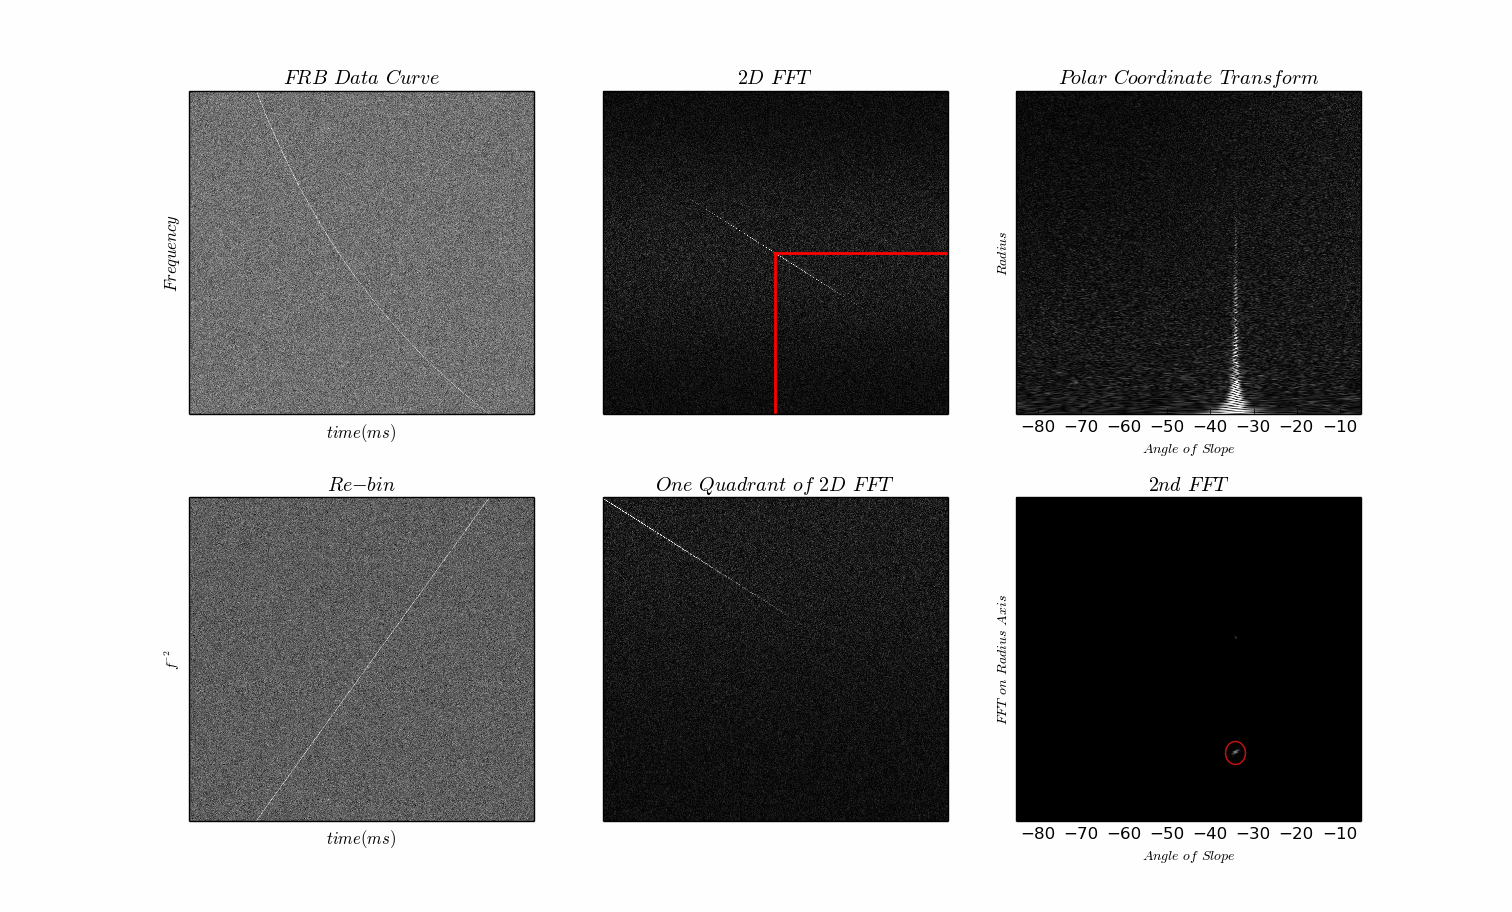
\includegraphics[width=180mm]{./pictures/procedure1.png}
\caption{The whole process of 2DFFT algorithm. Left top is Raw data of FRB data curve in $f(t)$ form which are follow Eq(\ref{eq:Disperse relation}). Left bottom is Re-bin process on Raw data,after this process curve in the Left top will comes to a straight line in $f^{-2}(t)$ form. Mid top is Re-bin Data after 2D FFT. Straight line in Left bottom turn into a straigt line that rotate 90$^{\circ}$ and go through center. As discussed in Sec \ref{sec:polar coordinate transform}, we could only take one quadrant data. Here we take data inside red line area of Mid top. One quadrant data are showed in Mid bottom. In Mid bottom image, Left top point is taken as origin and top horizontal line as origin axis, Then calculate the radius and angle of slope of each pixel and change this image into polar coordinate image of $(radius,angle)$ form as showed in Right top. As phase term influence, interference 	texture could be found on 2D FFT image. Then final step is doing 1D FFT along radius axis on polar coordinate data, then entire signal line will converge to several spots as showed in Right bottom.  \label{fig:Procedure}}
\end{figure*}

\subsection{polar coordinate transform}\label{sec:polar coordinate transform}

As DM always bigger than zero, so $k_2$ is always positive. It indicate signal after 2D-FFT is a straight line which will only appear in 1/2 of 2DFFT map. For example, Fig.\ref{fig:2DFFT} shows a signal line location after 2DFFT, it won't show up in quadrant \uppercase\expandafter{\romannumeral2} and  \uppercase\expandafter{\romannumeral4}, but only quadrant \uppercase\expandafter{\romannumeral1} and \uppercase\expandafter{\romannumeral3}. nevertheless quadrant \uppercase\expandafter{\romannumeral1} and \uppercase\expandafter{\romannumeral3} are conjugate to each other, we can only take 1 of them.

\begin{figure}
\epsscale{1}
\plotone{./pictures/1stFFT.png}
\caption{Signal on 2DFFT map \label{fig:2DFFT}}
\end{figure}

For purpose of search transient on 2D-FFT map, we need trace every slope of line which go cross center. It's easier to get each straight which pass through center from raius and angle of slope space $(r,\theta)$. Thus it's better to take a coordinate transform.  In Fig. \ref{fig:2DFFT},  If we make use of quadrant \uppercase\expandafter{\romannumeral1}, we can take map center as origin $O$, and horizontal axis as original axis, then each line go cross center will have radius and angle information. 

%It's not necessary to take the whole quadrant \uppercase\expandafter{\romannumeral1}, like the yellow part can be cast off. Because signal line go through 2DFFT will be not that long. Data after 2DFFT are in shape of square, $[N_{ch},N_t]$ for example, we can take the radius as ${\min(N_{ch}/2,N_t/2)}$ when we do polar coordinate transform. There are a lot of ways to take polar coordinate transform. But here we are taking interpolation which might be more smooth. After polar coordinate transform, signal line will exist at some exact angle $\theta$. As shows in right top of Fig \ref{fig:Procedure}. 

As tiny scale before FFT will decide large structure after FFT. Taking care of direction of FFT, Signal length in 2D-FFT map depend on width of signal line on re-bin map. Similarly, For polarization coordinates transform, the angle resolution could get from the length of signal line on re-bin map.  Note width and length of signal before 2D-FFT is $w_s$ and $l_s$, the length and width of signal after 2D-FFT will be $l_{FFT}=1/w_s$ and $w_{FFT}=1/l_s$ separately. Dimension of pixel need to be considered when actually process.
Thus It's not necessary to take the whole data of quadrant \uppercase\expandafter{\romannumeral1} but pixels whose radius value smaller tan $l_{FFT}$.  Furthermore, if $DM$ range are already set up, the boundary angle of slope $[\theta_{DM_{min}},\theta_{DM_{max}}]$ are also been decided according to Eq \ref{seq:DM Calculate}.  Thus pixel whose angle of slope are beyond boundary could be cast through.
%Actually,  if DM range is given, only small part of data are useful and 
%Because length of signal after 2D-FFT will be shortened.  That Data after 2DFFT are in shape of square, $[N_{ch},N_t]$ for example, we can take the radius as ${\min(N_{ch}/2,N_t/2)}$ when we do polar coordinate transform. 

There are a lot of ways to take polar coordinate transform. But here we are taking interpolation which might be more smooth. 
%Interpolation algorithm are showed on Algorithm I.
%\begin{algorithm}[H]
%\caption{The Interpolation Algorithm}
%\label{interpolation}
%Input: Data after FFT denote in $\mathcal{F}(f^{-2},t)$ whose shape assume to be $[N_{chan}, N_{samp}]$; $DM$ range that observer want to search; Reasonable width of pulse:$w_s$, Generally take minimum width                                                 value from FRB already known. 
%
%Output: Polar coordinate data denote in $\mathcal{P}(r,\theta)$. Shape of data is $[N_r,N_{\theta}]$.
%
%\begin{algorithmic}
%  %\scriptsize
%  \STATE Calculate $\theta$ boundary and $r$ range from given 
%  
%  \FOR{iteration $i=1$ to $i=log_2{N_f}$}
%  \FOR{$f_0$ in the range $\left[f_{\min},f_{\max}\right]$ with steps $2^i\delta_f$}
%   
%  \STATE $f_2 = f_0 + 2^i\delta_f$
%  \STATE $f_1 = \frac{f_2 - f_0}{2}$
%  \STATE $C_{f_2,f_0} = \frac{f_1^{-2} - f_0^{-2}}{f_2^{-2} - f_0^{-2}}$
%  \STATE $\Delta t_{\max}(i,f_0) = N_\Delta \frac{f_0^{-2} - (f_0 + 2^i\delta_f)^{-2}} {f_{\min}^{-2} - f_{\max}^{-2}} $
%  \FOR{$\Delta t$ in the range $[0,\Delta t_{\max}(i,f_0)]$}
%  \FOR{$t_0$ in range $[C_{f_2,f_0} \Delta t,N_t]$}
%  \STATE $t_1 = t_0 - C_{f_2,f_0}\Delta t$
%  \STATE
%  $
%  A_{f_0}^{f_2}(t_0,\Delta t) = A_{f_0}^{f_1}(t_0,t_0-t_1) + A_{f_1}^{f_2}(t_1,t_1-t_2)
%  $
%  \ENDFOR
%  \FOR{$t_0$ in the range $[0,C_{f_2,f_0} \Delta t]$}
%    \STATE
%    $
%    A_{f_0}^{f_2}(t_0,\Delta t) = A_{f_0}^{f_1}(t_0,C_{f_2,f_0} \Delta t)
%    $
%    \ENDFOR
%    
%  
%  \ENDFOR
%  \ENDFOR 
%  \ENDFOR
%  
%\end{algorithmic}
%\end{algorithm}

 After polar coordinate transform, signal line will exist at some exact angle $\theta$. As shows in right top of Fig \ref{fig:Procedure}. 

\subsection{Turn signal line into spot}
As we discussed before, the phase term $e^{-i2\pi vb}$ could disturb the signal. Since phase term is monotonically and data are complex number, if we integrate along radius directly, signal intensity will be blended. We also can't take absolute value then sum,  due to noise will be amplified. A reasonable method is to take another FFT along radius axis, so that the influence of phase term will be eliminated.
After this we could get Signal Noise Ratio by 
\begin{equation*}
SNR = \frac{Max~Value }{std}
\end{equation*}
When we know where the highest SNR is , we can got the slope of it , finally calculate the DM value from Eq.(\ref{seq:DM Calculate}). 
The entire procedure are showed by Fig\ref{fig:Procedure}. Data are generated by SIGPROC $fake$ command and parameter are simulated from TianLai Array FRB backend request which Time resolution is 0.1 millisecond, Band width is 100 MHz and central Frequency is 750 Mhz,  with 2048 Frequency Channels.




\section{Detection of observed FRB data}
Observed FRB data are tested through this algorithm. 
%\section{Compute Complexity and benchmark}

\section{Incoherent De-dispersion Algorithm Analysis}
There are a lot of incoherent transient search algorithm already in use, But I'd like to difference them into three types: $brute~force$ , $tree$ ,  $image~processing$,$machine~learning$. \\

%\subsection{Algorithm Compute Complexity}

\subsubsection*{brute force}
$Brute~force$ is implemented in a lot of software like SIGPROC, HEIMDALL. In general, the compute complexity of transient search algorithm is compute dependency on number of time samples $'N_t'$, number of frequency channels $'N_{\nu}'$ and number of DM $'N_{DM}'$ of observation. The basics of $brute~force$ is to shift time delays back for each frequency channel according to Eq\ref{eq:Disperse relation}. As every DM are processed with every time sample and frequency channel, so the total compute complexity is $(N_t N_{\nu} N_{DM})$. It has the slowest compute complexity along the 3 types, However it is easier to parallel and implement on GPUs which are good at high performance computing. HEIMDALL is an example to take use GPU to De-disperse. It has been used for a lot of real-time survey like UTMOST \ref{} and ??? and already detected lots of FRB instances. It's also the one who has best compatibility for phase of pulses.   \\

\subsubsection*{tree}
Different with $brute~force$ algorithm, Talor proposed $tree$ algorithm \ref{} to accelerate $brute force$ de-disperse algorithm. Under assumption of Eq \ref{eq:linear assumption}, Tree algorithm trace signal across a straight line and reuse some element to get rid of redundant calculation. It has same mechanism as FFT and compute complexity is $(N_t N_{\nu} \log_2{N_{\nu}})$.	Though Tree algorithm is much faster than $brute~orce$, it is difficult at piratical application. The result are iterative at each step, This algorithm has worse  parallelism. Signal line are approximate linear, so tree algorithm also have detective sensitivity loss problem. Advanced 'tree' method are brought out. People are using sub frequency band to get curve more like straigt and thus parallel compute could be achieved. Moreover, $FDMT$ algorithm are proposed to get accurate curve calculated in decent subband \ref{}. In $FDMT$ algorithm, the compute complexity is $\max \{N_tN_{DM}\log_2(N_{\nu}),2N_{\nu}N_t\}$.\\

\subsubsection*{2DFFT}
Algorithm discussed in this paper is kind of $image~processing$ way to De-disperse. This type of algorithm focus on finding a signal line on given $(f,t)$ data. Except algorithm talked in this paper, there are a lot of ways to accomplish this algorithm, like radon transform and machine learning. The compute complexity is varied with different implement method. For 2D-FFT algorithm talked in this paper, The most time consuming step is 2D-FFT. Though second 1-D FFT are executed on $(r,\theta)$ data, this doesn't change complexity due to $N_t$,$N_{\nu}$, or $N_{DM}$. Because data shape after polar coordinate transform is only decided by supposed signal width $w_s$ and assumed signal length $l_s$ which are constant during a observation. The scale need to process are much smaller than 2D-FFT . Thus the compute complexity got from this algorithm are mainly caused by 2D-FFT which are $2N_t N_{\nu} \log_2(N_t N_{\nu})$. \\

\begin{deluxetable*}{lcccc}[H]  % <--- column justification (center/left/right)
\tablecolumns{5}
\tablecaption{Algorithm comparison \label{AlgorithmComparisonTable}}
\tablehead{   % column headings
  \colhead{} &
  \colhead{2DFFT} &
  \colhead{Brute force} &
  \colhead{Tree} &
  \colhead{FDMT} 
}
\startdata
Computational complexity & $2N_t N_{\nu} \log_2(N_t N_{\nu})$ & $N_{\nu}N_tN_{DM} $& $N_{\nu}N_t\log_2(N_{\nu})$ & $\max\{N_tN_{DM}\log_2(N_{\nu}),2N_{\nu}N_t\}$ \\
DM smearing & No & Yes & Yes & Yes \\
Parallelization friendly & Yes & Yes & No & Yes
\enddata
\end{deluxetable*}


2DFFT algorithm doesn't have simplest compute complexity.  Take Tree algorithm for example, this method will twice the complexity.  However there are some advantages that we might be interested. No matter $brute~force$ or $tree$ algorithm, DM smearing problem can't be get rid off. Because the signal line go through more than 1 time sample at single frequency channel at higher DM value. But in image processing way to de-disperse, we are searching a line in the graphic, so that DM smearing problem could be solved. Thereby we might achieve higher detective sensibility. For pulsar transient searching, this algorithm also include the folding step, as pulses have same DM value and will shows in the same location after 2DFFT. Parallel process are also compatible for 2DFFT algorithm, we could cut $[N_{\nu},N_t]$ data along time axis into $N_{thread}$ data chunks of shape $[N_{\nu},N_t^{'}]$. Note $N_t^{'}$ might not big enough to ensure signal line at largest DM value locate in single data chunk, Then an extra search along slope should be implemented.  Table \ref{AlgorithmComparisonTable} shows comparison with some transients search algorithm like $brute~force$, $tree$, $FDMT$.  
	Previous work Ait-Allal find this algorithm has great advantage on RFI mitigation, but in this paper , We found Sensitivity is also remarkable. We take 




\subsection{Benchmark between different Algorithms}
\begin{figure}[ht!]
\epsscale{1}
\plotone{./pictures/benchmark.png}
\caption{Benchmark of Transient search software: Sigproc, Sigpyproc, Heimdall , 2DFFT \label{fig:benchmark}}
\end{figure} 
This 

\subsection{Advantage on RFI removing}
There are two sorts of regular RFI: At certain frequency last long time, At certain time stamp but with large bandwidth, corresponding to horizontal and vertical line separately in image of Re-bin data. After 2D FFT , they will rotate 90$^{\circ}$, but all of them go through center no matter what frequency or time stamp they are. Therefore, Regular type of RFI could be removed simply by discarding data after 2D FFT at horizontal and vertical line that go cross center.%0$^{\circ}$ and -90$^{\circ}$. 
An example could be seen from Fig. \ref{fig:RFI remove}.

\section{Discussion}

\begin{figure}[ht!]
\centering
\subfigure[Add RFI manually on Re-bin map]{
\epsscale{1.1}
\plotone{./pictures/RFI_remove-1.png}
}
\subfigure[RFI are removed on 2D FFT map]{
\plotone{./pictures/RFI_remove-2.png}}
\caption{Plot (a) shows Re-bin map which are add 3 RFI manully: Time domain and frequency domain and short bad data area. Seeing from Plot (b), RFI are removed clearly.  \label{fig:RFI remove}}
\end{figure}


	

 




\begin{thebibliography}{}
\expandafter\ifx\csname natexlab\endcsname\relax\def\natexlab#1{#1}\fi

%\bibitem[Bannister \& Cornwell(2011)]{Chirpolator} Bannister, K.~W., \& Cornwell, T.~J.\ 2011, \apjs, 196, 16

\bibitem[Barsdell et al.(2012)]{GPUDedispersion} Barsdell, B.~R., Bailes, M., Barnes, D.~G., \& Fluke, C.~J.\ 2012, \mnras, 422, 379  

\bibitem[Brady (1998)]{RadonBrady}
 Brady, Martin L. "A fast discrete approximation algorithm for the Radon transform." SIAM Journal on Computing 27, no. 1 (1998): 107-119.

\bibitem[Clarke et al.(2013)]{FPGADedispersion} Clarke, N., Macquart, J.-P., \& Trott, C.\ 2013, \apjs, 205, 4 

\bibitem[Clarke et al.(2014)]{DedispersionInterferometers} Clarke, N., D'Addario, L., Navarro, R., \& Trinh, J.\ 2014, Journal of Astronomical Instrumentation , 3, 50004 


\bibitem[Gotz \& Druckmuller(1996)]{RadonGotsDruckmuller}	Gotz, W. A., and H. J. Druckmuller. "A fast digital Radon transform. An efficient means for evaluating the Hough transform." Pattern Recognition 29, no. 4 (1996): 711-718.


\bibitem[Manchester et al.(1996)]{sub-bandDedispersion} Manchester, R.~N., 
Lyne, A.~G., D'Amico, N., et al.\ 1996, \mnras, 279, 1235


\bibitem[Magro et al.(2011)]{GPUsub-bandDedispersion} Magro, A., Karastergiou, 
A., Salvini, S., et al.\ 2011, \mnras, 417, 2642


\bibitem[McLaughlin 
\& Cordes(2003)]{DetectingPulsarsByGiantPulses} McLaughlin, M.~A., \& Cordes, J.~M.\ 2003, \apj, 596, 982 

\bibitem[Lorimer et al.(2007)]{LorimerBurst} Lorimer, D.~R., Bailes, 
M., McLaughlin, M.~A., Narkevic, D.~J., 
\& Crawford, F.\ 2007, Science, 318, 777

\bibitem[Lorimer 
\& Kramer(2012)]{HandbookOfPulsarAstronomy} Lorimer, D.~R., \& Kramer, M.\ 2012, Handbook of Pulsar Astronomy, by D.~R.~Lorimer , M.~Kramer, Cambridge, UK: Cambridge University Press, 2012,

\bibitem[Petroff et al.(2014)]{PetroffFRBsNullDetection} Petroff, E., van 
Straten, W., Johnston, S., et al.\ 2014, \apjl, 789, L26  

\bibitem[Taylor(1974)]{TreeDedispersion} Taylor, J.~H.\ 1974, \aaps, 15, 367 

\bibitem[Thompson et al.(2011)]{DedispersionInterferometersCaseStudy} Thompson, D.~R., Wagstaff, K.~L., Brisken, W.~F., et al.\ 2011, \apj, 735, 98 

\bibitem[Thornton et al.(2013)]{FRBS} Thornton, D., 
Stappers, B., Bailes, M., et al.\ 2013, Science, 341, 53

\bibitem[van Leeuwen \& Stappers(2010)]{LOFARPulsar}
 van Leeuwen, J., \& Stappers, B.~W.\ 2010, \aap, 509, A7


\end{thebibliography}

\end{document}


